\documentclass{article}

\usepackage[a4paper]{geometry} 
\usepackage[dutch]{babel} % Juiste afbreekregels en dergelijke!
\usepackage{parskip} % Alinea's beginnen links uitgelijnd en er staat een lege regel tussen alinea's.
\usepackage{amsmath, amssymb, textcomp} % Wiskundige symbolen e.d.
\usepackage{color} % Kleuren
\usepackage{graphicx} % Plaatjes
\usepackage{enumerate} % Voor opsommingen
\usepackage[official]{eurosym}
\usepackage{url} % Voor het weergeven van hyperlinks
\usepackage{float}
%\usepackage{minted} % Voor source-code weergeven
\usepackage{gensymb}
\usepackage[hidelinks]{hyperref} % Voor clickable links van refs
\usepackage[nottoc,numbib]{tocbibind} % Om de referenties in de inhoudsopgave te krijgen

\setcounter{secnumdepth}{0} % Om ervoor te zorgen dat er geen hoofdstuknummers voor de hoofdstuktitels komen

\title{Testverslag ATP\\
		   Lemonator}
\author{Philippe Zwietering\\
	           Studentnummer: 1685431}
           
\begin{document}
	\maketitle
      	
    \clearpage
    
    \section{Inleiding}
    
    In dit document wordt besproken welke tests zijn uitgevoerd voor het ATP lemonator project en welke kwaliteit die hadden om de zekerheid van dit project te waarborgen. Het beschrijft ook in welke mate er is afgeweken van het testplan.
    
    \section{Gebruikte infrastructuur} 
    Tijdens het project is gebruik gemaakt van bepaalde tools voor het automatiseren en analyseren van de tests en van tools voor het algemeen bevorderen van het projectverloop.
    
    \subsection{Tools}
    Voor dit project is gebruikgemaakt van git als versiebeheer met GitHub als serverplatform. Op die manier kon enigszins zeker worden gesteld dat alle versies correct worden beheerd op een externe server, ook al heb ik dit project in mijn eentje uitgevoerd. 
    
    Dit project is voornamelijk geschreven in Python 3.7 en op een gegeven moment is er ook gebruikgemaakt van C++ 11+ voor het schrijven van de C++ Controller. Het project is geschreven op een 64-bits Linux systeem. 
    
    Om tests uit te voeren is gebruikgemaakt van het nose2 package van Python. nose2 maakt gebruik van het unittest package, wat een vrij standaard manier is om tests op te stellen. nose2 kan automatisch alle tests in een map zoeken en uitvoeren, met ondersteunende functionaliteit voor setUps zodat bepaalde code opgezet kan worden voor alle tests van dezelfde smaak zodat dit niet iedere keer opnieuw hoeft worden geschreven. Om dit uit te voeren typt men nose2 in de betreffende map. Het enige waar voor gezorgd moet worden is dat alle testklasses en functies beginnen met test, de rest gebeurt vanzelf.
    
    Om de coverage van de Pythontests te meten wordt gebruikgemaakt van de coverage module van Python. Deze kan rapporten genereren voor de coverage van de tests, zodat kan worden gecheckt dat ten minste alle code afgegaan wordt in de hoop dat alle aspecten van de code ook getest wordt. Om een coverage report te geven van de tests van nose2 kan nose2 --with-coverage worden uitgevoerd op de command line in de relevante map.
    
    Verder wordt er voor het C++ gedeelte van de opdracht gebruikgemaakt van Pybind11 en cppimport, een Python module die het makkelijker maakt om pybind11 te gebruiken. Dit scheelt enorm veel werk en gedoe met buildfiles en CMake. Het is voor het builden van dit project dus nodig dat de volgende modules en libraries van tevoren goed worden ge\"installeerd: coverage, nose2, unittest, cppimport en als C++-dependency pybind11.
    
    \subsection{Mappenstructuur}
    Uiteindelijk is voor dit project alleen de simulatormap gebruikt. Ik weet dat dit niet netjes is, maar wegens tijdgebrek en wegens gemakzucht heb ik ervoor gekozen om alle Python code in dezelfde map te zetten, zodat ik niet moeilijk hoefde te doen met de sys.path, wat me aardig wat hoofdpijn bezorgde in het begin van dit project. Ook de C++-controller staat in deze map, zodat makkelijk ge\"importeerd en ge\"exporteerd kan worden. Al deze code staat in de simulator map, de overige mappen worden door de student niet gebruikt.
    
    \section{Reproduceerbaarheid tests}
    Voor de tests wordt dus gebruikgemaakt van nose2 en unittest. Het unittesten gebeurt hierdoor op een gestandaardiseerde manier, en sommige integration tests die niet handmatig moeten worden gecontroleerd kunnen op een gelijkwaardige manier gebeuren. De unittests zijn namelijk allemaal op dezelfde manier opgebouwd: ze vallen in een bepaalde TestCase klasse die alle mogelijke functies hoort af te gaan voor een bepaalde klasse van de code. In de setUp functie van de TestCase klasse wordt alle code geschreven die alle tests nodig hebben van die klasse. Zie de afbeelding voor een voorbeeld. Deze setUp code wordt voor iedere testfunctie opnieuw uitgevoerd, dus er is geen onderline afhankelijkheid. Zoals ook te zien is wordt er getest door middel van asserts: faalt deze dan faalt de test. Dit wordt gebruikt om variabelen langs te gaan die relevant worden geacht voor de unittest en te checken of die de waarden hebben die ze zouden moeten hebben.
    
    Om de tests uit te voeren kan nose2 worden uitgevoerd in de command line in de simulator map. Alle tests die zijn geschreven met behulp van unittest worden dan langsgegaan.
    
    \begin{figure}[H]
    	\centering
    	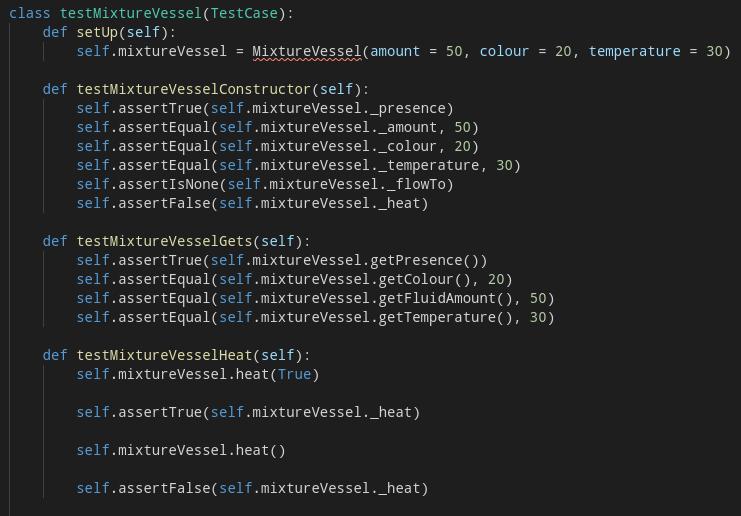
\includegraphics[width=0.9\textwidth]{figures/setup.png}
    	\caption{Voorbeeld unittest (er zijn er nog meer voor deze klasse)}
    \end{figure}

	\section{Test verantwoording}
	Er zijn voor dit project uiteindelijk vooral unittests geschreven. Wegens tijdgebrek vanwege problemen met pybind11 ben ik nauwelijks toegekomen om systemtests te schrijven. Het grootste gedeelte van de tests die dus wel wordt uitgevoerd zijn whitebox unittests op de plant, de CustomController wordt nauwelijks gecheckt. Dit is uiteraard geen goede dekking en is dus eigenlijk niet nuttig als test coverage.
	
	Qua unittests zijn er voornamelijk 2 typen tests: een bestand checkt via mocks de SimulatorProxy en een bestand checkt alle functionaliteit van de plant van de simulator. De SimulatorProxy wordt dus alleen gecheckt op het uitvoeren van de corresponderende functies van de plant, omdat de functionaliteit alleen maar gecheckt hoeft te worden bij de daadwerkelijke simulatie. Het is vrij belangrijk om unittests uit te voeren voor de plant, omdat dan kan worden gecontroleerd dat fouten in de Controller niet toevallig veroorzaakt worden door een waarde die verkeerd wordt uitgelezen of doorgegeven.
    
\end{document}}